\documentclass{beamer}

\usepackage[utf8]{inputenc}
\usepackage{color, xcolor}

\usepackage{multicol}
\usepackage{fancyhdr}
\usepackage{listings}
\usepackage{graphicx, subfig}
\usepackage{float}
\usepackage{enumerate}

\usepackage{amsfonts}
\usepackage{eucal}
\usepackage{amsmath}
\usepackage{amssymb}
\usepackage{gensymb}
\usepackage{amsthm}
\usepackage{makecell}
\usepackage[ruled]{algorithm2e}
\usepackage{tikz}
\usetikzlibrary{positioning}

\usepackage[backend=bibtex,style=authoryear]{biblatex}
\bibliography{reference.bib}
\setbeamerfont{footnote}{size=\tiny}
\renewcommand{\thefootnote}{[\arabic{footnote}]}

\title{Project Report}
\author{Team \#12}
\institute{
  \parbox{0.2\textwidth}{
    \centering WANG Zeyu \\
    \vspace{.25cm}
    \centering 24056788G
  }
  \parbox{0.2\textwidth}{
    \centering YANG Xirui \\
    \vspace{.25cm}
    \centering 24135668G
  }
  \parbox{0.2\textwidth}{
    \centering Wu Tianxiao \\
    \vspace{.25cm}
    \centering 24084591G
  }
}
\date{\today}

\usetheme{Madrid}
\usecolortheme{default}
\setbeamertemplate{navigation symbols}{}

\setbeamertemplate{footline}
{
  \leavevmode%
  \hbox{%
  \begin{beamercolorbox}[wd=0.3\paperwidth,ht=2.25ex,dp=1ex,center]{author in head/foot}%
    \usebeamerfont{author in head/foot}\insertshortauthor
  \end{beamercolorbox}%
  \begin{beamercolorbox}[wd=.4\paperwidth,ht=2.25ex,dp=1ex,center]{title in head/foot}%
    \usebeamerfont{title in head/foot}\insertsection
  \end{beamercolorbox}%
  \begin{beamercolorbox}[wd=0.3\paperwidth,ht=2.25ex,dp=1ex,center]{date in head/foot}%
    \usebeamerfont{date in head/foot}\insertshortdate{}\hspace*{2em}
    \insertframenumber{} / \inserttotalframenumber\hspace*{2ex}
  \end{beamercolorbox}}%
  \vskip0pt%
}

\usefonttheme[onlymath]{serif}

\begin{document}

\section*{Cover}
\frame{\titlepage}

\section*{Contents}
\begin{frame}{Contents}
  \tableofcontents
\end{frame}

\section{Problem definition}

\begin{frame}{Problem definition}

  \begin{itemize}
    \item \textbf{Task 1}: Train models based on $10$ features, including academic metrics, aptitude scores, and soft skill ratings, to predicting whether a student will be successfully placed in a job. \vspace{.25cm}
    \item \textbf{Task 2}: Train models based on $18$ anonymity features and labeled with $5$ classes, then predict the labels based on the training set. \vspace{.25cm}
    \item \textbf{Task 3}: Train models based on $28$ anonymity numerical with the transaction amount, to indicate whether it is a fraudulent transaction or a legitimate transaction. \vspace{.25cm}
  \end{itemize}

\end{frame}

\section{Method}

\subsection{Data Prepare}

\begin{frame}{Correlation coefficient \footfullcite{abdi2007kendall} \footfullcite{hauke2011comparison}}

  \begin{itemize}
    \item \textbf{Pearson correlation coefficient}: Measures linear correlation between two sets of data; \vspace{.25cm}
    \item \textbf{Kendall correlation coefficient}: Measures the rank correlation by counting the concordant pairs; \vspace{.25cm}
    \item \textbf{Spearman correlation coefficient}: Measures the rank correlation based on the Pearson correlation coefficient; \vspace{.25cm}
  \end{itemize}

\end{frame}

\begin{frame}{$k$-nearest neighbors imputer \footfullcite{troyanskaya2001missing} \footfullcite{juna2022water}}

  The $k$-nearest neighbors imputer estimating the missing values using the $k$ nearest neighbors which: \vspace{.25cm}

  \begin{itemize}
    \item Works with both numerical and categorical data; \vspace{.25cm}
    \item Don't need any assumption about the data distribution; \vspace{.25cm}
    \item Is robust in many applications. \vspace{.25cm}
  \end{itemize}

\end{frame}

\begin{frame}{Dimension raising}

  Given the scalar data $x_i$ and a given degree $d$, we compute the new data as

  $$
    (x_i, x_i^2, \dots, x_i^d).
  $$

  \begin{figure}[H]
    \centering
    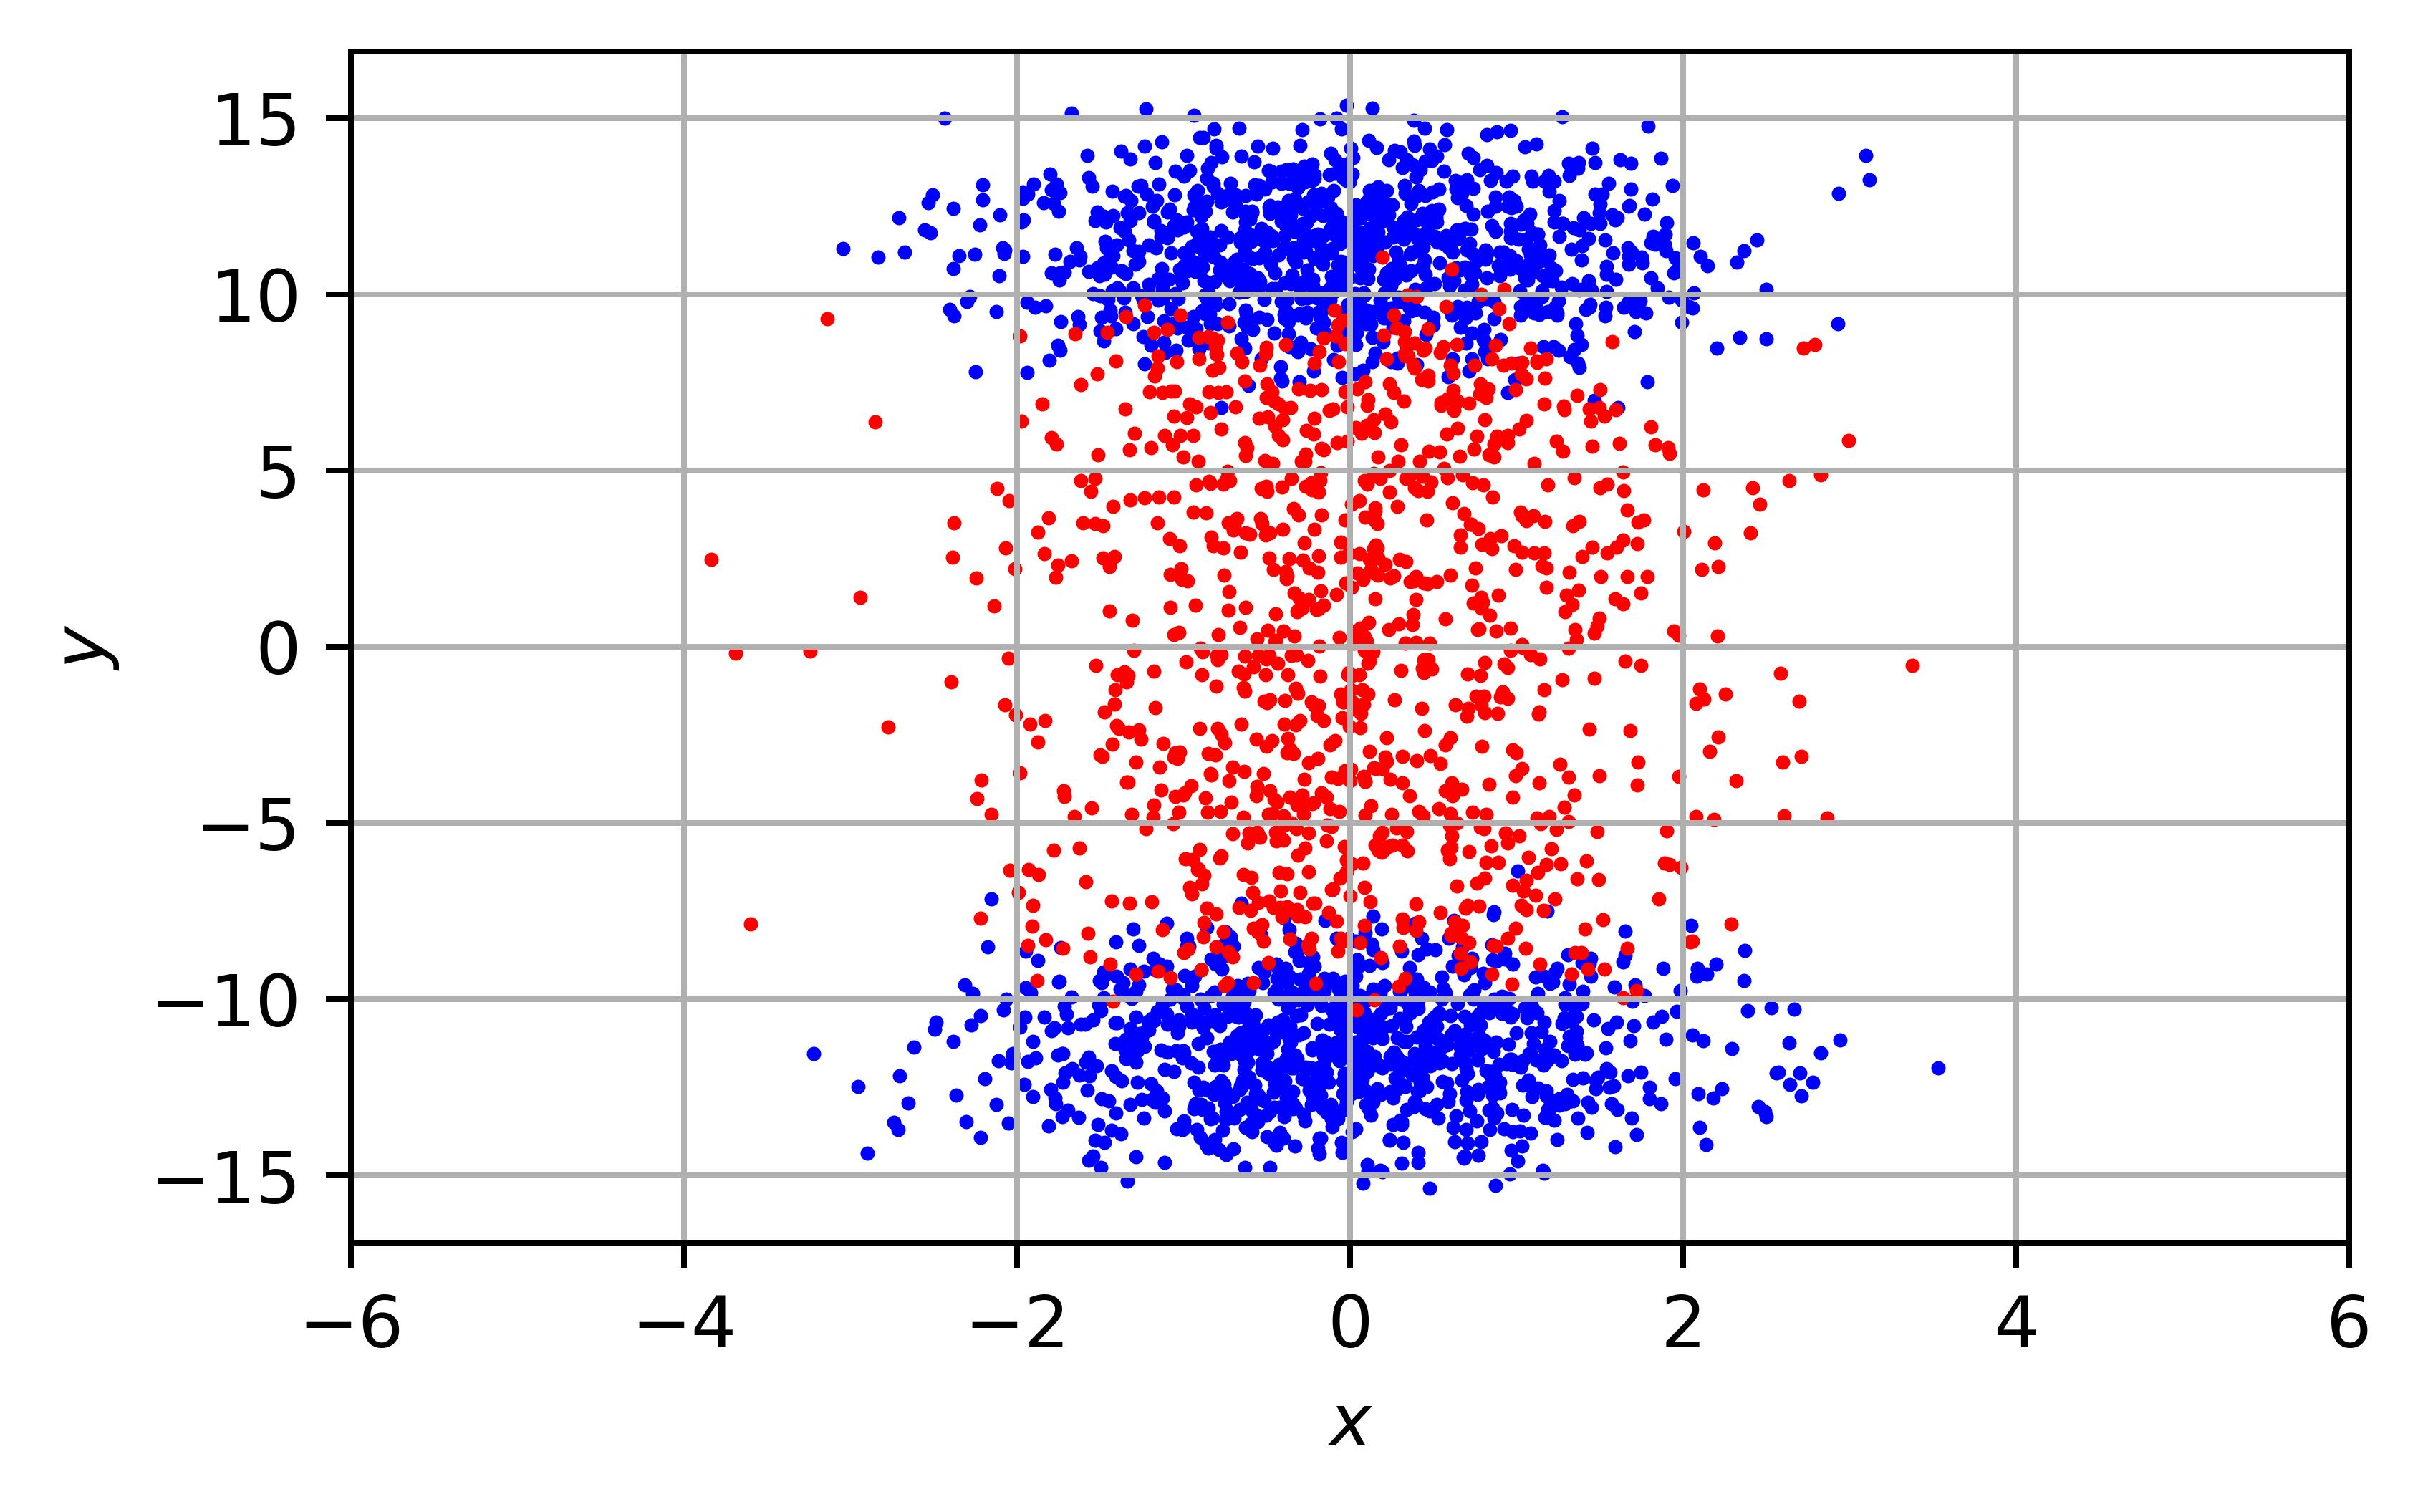
\includegraphics[width=0.4\textwidth]{./figure/Sample-Raising-1.jpg}
    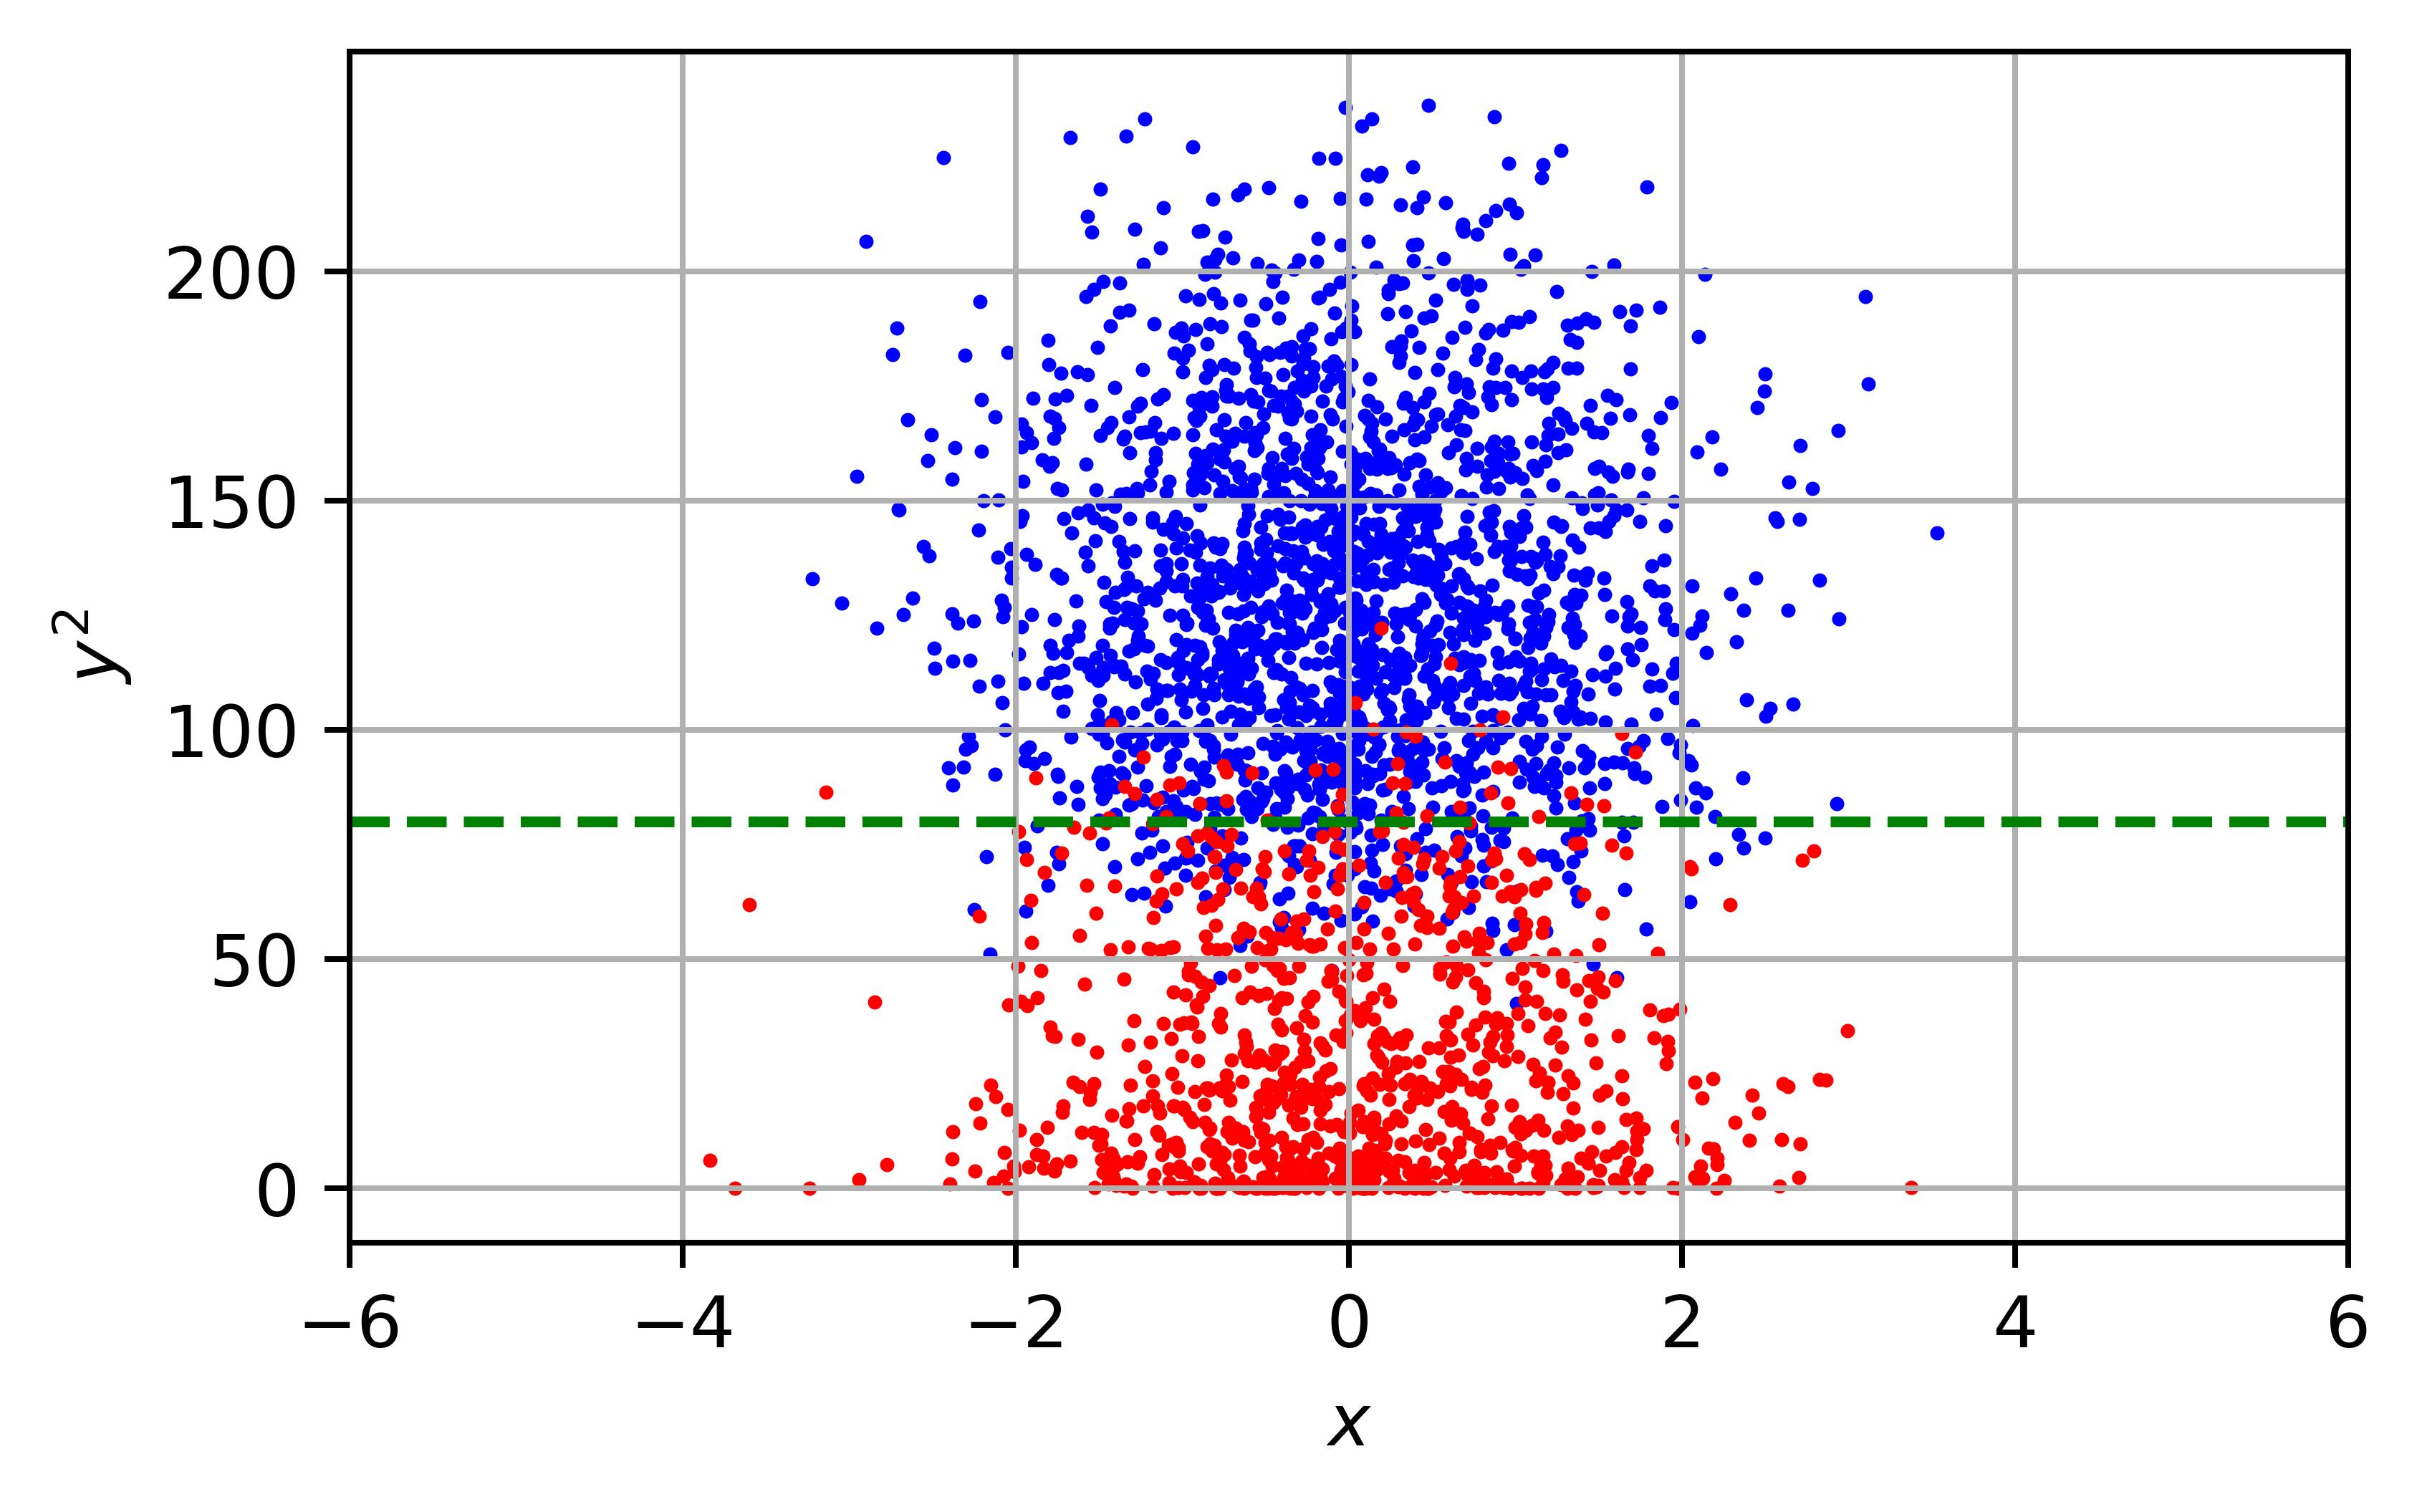
\includegraphics[width=0.4\textwidth]{./figure/Sample-Raising-2.jpg}
    \caption{Example for dimension raising. The left shows that origin data is not linearly separable, while the right shows the data after dimension raising, where the $y_2$ is easy to be linearly separated.}
  \end{figure}

\end{frame}

\begin{frame}{Dimension raising}

  For the meaningful features, we can do the dimension raising manually, e.g., in task 1, \vspace{.25cm}

  \begin{itemize}
    \item Internships, Projects, Workshops/Certifications $\Longrightarrow$ Practice; \vspace{.25cm}
    \item AptitudeTestScore, SoftSkillsRating $\Longrightarrow$ Potential Ability; \vspace{.25cm}
    \item SSC\_Marks, HSC\_Marks $\Longrightarrow$ Progress. \vspace{.25cm}
  \end{itemize}

\end{frame}

\subsection{Data Analysis}

\begin{frame}{Data Analysis}

  \begin{itemize}
    \item \textbf{The logistic regression} \footfullcite{walker1967estimation} \footfullcite{pohar2004comparison} is a widely used linear classification model, which gives a probability value ranging between $0$ and $1$; \vspace{.25cm}
    \item \textbf{The decision tree} \footfullcite{utgoff1989incremental} \footfullcite{kotsiantis2013decision} is a supervised learning method used for classification which predict the label with piecewise constant approximation; \vspace{.25cm}
    \item \textbf{The multilayer perceptron (MLP)} \footfullcite{rosenblatt1958perceptron} \footfullcite{rumelhart1986learning} is a basic kind of neural network which learns a function $f: \mathbb{R}^n \mapsto \mathbb{R}^m$ to approximate the input and output, with the ability of hierarchical feature extraction.
  \end{itemize}

\end{frame}

\section{Solution}

\begin{frame}{Solution Overview}

  \begin{figure}[H]
    \centering
    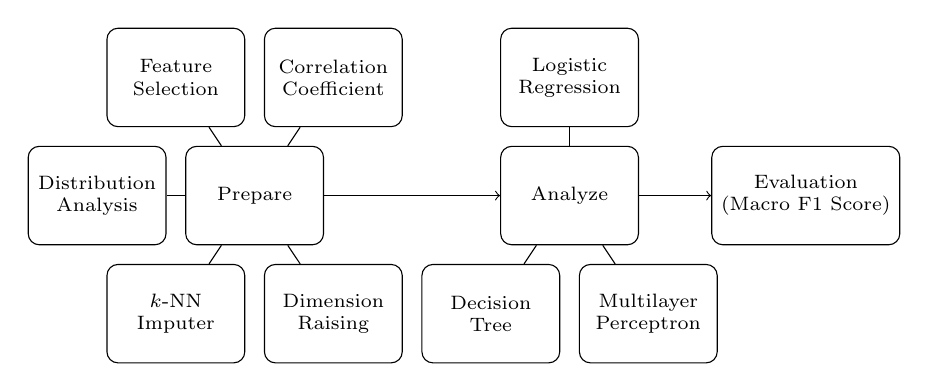
\begin{tikzpicture}[minimum width=1.75cm, minimum height=1.25cm, font=\scriptsize]
      \node[draw, align=center, rounded corners]  (P)   at ( 0,  0.0)    {Prepare};
      \node[draw, align=center, rounded corners]  (DA)  at (-2,  0.0)    {Distribution \\ Analysis};
      \node[draw, align=center, rounded corners]  (CC)  at ( 1,  1.5)    {Correlation \\ Coefficient};
      \node[draw, align=center, rounded corners]  (FS)  at (-1, 1.5)     {Feature \\ Selection};
      \node[draw, align=center, rounded corners]  (DR)  at ( 1, -1.5)    {Dimension \\ Raising};
      \node[draw, align=center, rounded corners]  (KNN) at (-1, -1.5)    {$k$-NN \\ Imputer};

      \node[draw, align=center, rounded corners]  (A)   at ( 4,  0.0)    {Analyze};
      \node[draw, align=center, rounded corners]  (LR)  at ( 4,  1.5)    {Logistic \\ Regression};
      \node[draw, align=center, rounded corners]  (DT)  at ( 3, -1.5)    {Decision \\ Tree};
      \node[draw, align=center, rounded corners]  (MLP) at ( 5, -1.5)    {Multilayer \\ Perceptron};

      \node[draw, align=center, rounded corners]  (E)   at ( 7,  0.0)    {Evaluation \\ (Macro F1 Score)};

      \draw[->] (P) -- (A);

      \draw[-]  (P) -- (DA);
      \draw[-]  (P) -- (CC);
      \draw[-]  (P) -- (FS);
      \draw[-]  (P) -- (DR);
      \draw[-]  (P) -- (KNN);

      \draw[-]  (A) -- (LR);
      \draw[-]  (A) -- (DT);
      \draw[-]  (A) -- (MLP);

      \draw[->] (A) -- (E);
    \end{tikzpicture}
    \caption{Overview flowchart.}
  \end{figure}

\end{frame}

\section{Summary}

\begin{frame}{Discovery \& insights}

  \begin{itemize}
    \item The features engineering can help imrpove the model preformance, with the a higher time and memory cost; \vspace{.25cm}
    \item the effectiveness of feature engineering varies by task, which needs adjustments based on the data; \vspace{.25cm}
    \item The logistic regression preforms a better reliability and efficiency especially on linearly separable data, while MLP will be better in the complex multi-class problem; \vspace{.25cm}
    \item Regularization will reduce the influence of noise and outliers, which prevent the model from overfitting and ensuring the generalization; \vspace{.25cm}
    \item The parallel computing will significantly accelerate the training, but must be balanced against memory cost and convergence stability.
  \end{itemize}

\end{frame}

\begin{frame}{Future Work}

  \begin{itemize}
    \item Employ automated feature engineering tools insteal of manual design, which can improve feature selection and generation; \vspace{.25cm}
    \item Ensemble methods (e.g., random forests or gradient boosting trees) may help deal with the overfitting of decision tree; \vspace{.25cm}
    \item Adapt the models to the dynamic environment and input, especially can help detected the fraud in time; \vspace{.25cm}
    \item Use the distributed computing frameworks to speed up the model and also train with the large-scale datasets. \vspace{.25cm}
  \end{itemize}

\end{frame}

\section*{Reference}
\begin{frame}[allowframebreaks]{Reference}
  \printbibliography
\end{frame}

\appendix

\end{document}